% AURALIS -- IEEE conference draft.
% Build:  cd docs/paper && pdflatex auralis_ieee && pdflatex auralis_ieee
% Every number in this draft is produced by make_figures.py / routing_eval.mjs (see results.json).
% Orange [bracketed] text marks what still has to be measured or filled in before submission.
% Verify every reference against the original paper before submission.
\documentclass[conference]{IEEEtran}
\usepackage{graphicx}
\usepackage{amsmath,amssymb}
\usepackage{booktabs}
\usepackage{xcolor}
\usepackage{tikz}
\usetikzlibrary{positioning,arrows.meta,fit,backgrounds}
\usepackage[hidelinks]{hyperref}
\usepackage{cite}

\definecolor{tbd}{HTML}{C25400}
\newcommand{\tbd}[1]{\textcolor{tbd}{[#1]}}
\definecolor{cblue}{HTML}{2a78d6}
\definecolor{corange}{HTML}{eb6834}
\definecolor{caqua}{HTML}{1baf7a}

\begin{document}

\title{AURALIS: A Self-Mapping Smart Cane with Spatio-Temporal Hazard Memory and Neural Sensor Fusion for Visually Impaired Pedestrians}

\author{\IEEEauthorblockN{\tbd{Author 1}, \tbd{Author 2}, \tbd{Author 3}, \tbd{Guide name}}
\IEEEauthorblockA{\tbd{Department of \ldots}, \tbd{College name}, \tbd{City}, India\\
\tbd{email@college.edu}}}

\maketitle

\begin{abstract}
Electronic travel aids for visually impaired people are mostly reactive: they warn about an obstacle only while it is in front of the sensor and forget it immediately, although most daily walks repeat the same routes and meet the same hazards. We present AURALIS, a low-cost smart cane that \emph{remembers}. A Raspberry~Pi~4 on the cane runs a YOLOv8 convolutional detector on a USB camera and an HC-SR04 ultrasonic ranger, estimates distance from a single camera, and decides what to announce. The user's smartphone adds GPS and compass, speaks the alerts in English, Hindi, Telugu or Tamil through Bluetooth headphones, and maintains a spatio-temporal hazard memory: every hazard is stored at its estimated position, its risk grows with repeated sightings and decays with a seven-day half-life, and remembered hazards are announced up to 25\,m ahead, before they are visible. The phone also builds a pedestrian graph from the user's own walks, needing no map data, and plans routes with a risk-weighted A* search. A 484-parameter neural network fuses vision, ultrasonic and memory features into four alert levels with a hard safety override for drops. In this draft we report the implemented system and a preliminary evaluation: the fusion network reaches 0.890 accuracy and 0.933 urgent recall on a held-out synthetic set (rule baseline: 0.768 and 0.865), risk-aware routing cuts route risk by 89\% for a 2.2$\times$ longer path on a campus graph, and memory raises the warning lead time from about 2.5\,s to about 20\,s by design. Field experiments are planned and outlined.
\end{abstract}

\begin{IEEEkeywords}
assistive technology, smart cane, visually impaired navigation, object detection, YOLO, sensor fusion, spatio-temporal memory, risk-aware routing, edge AI
\end{IEEEkeywords}

% ---------------------------------------------------------------------------
\section{Introduction}
About 2.2 billion people live with a vision impairment, and at least 43 million are blind~\cite{who2019,bourne2017}. The white cane remains the most common mobility aid: it is cheap and reliable, but it only reaches about one metre ahead, at ground level. Electronic travel aids add ultrasonic or camera sensing~\cite{dakopoulos2010,elmannai2017,kuriakose2022}, and recent smart canes run deep object detectors such as YOLO~\cite{redmon2016} on embedded boards.

These systems share one limitation: they are \emph{reactive}. A pothole on the way to the library is detected only when it is a few metres away, every single day, and is forgotten as soon as it leaves the camera view. Yet a pedestrian's daily walks are highly repetitive, and the most dangerous hazards in Indian streets and campuses---open drains, potholes, broken steps, low branches---are static for days or weeks.

AURALIS turns the cane from a reactive sensor into a system that \emph{learns its user's environment}. Our contributions are:
\begin{enumerate}
\item \textbf{Spatio-temporal hazard memory} that combines repeated evidence with temporal decay and user correction, and warns about remembered hazards long before they come into view (Sec.~\ref{sec:memory}).
\item \textbf{Infrastructure-free self-mapping}: a pedestrian graph built from the user's own GPS breadcrumbs, with \textbf{risk-aware A*} routing on it (Sec.~\ref{sec:routing}).
\item \textbf{Neural late fusion} of camera, ultrasonic and memory features into a four-level alert, with a hard safety override (Sec.~\ref{sec:fusion}).
\item A \textbf{minimal, low-cost implementation}: one Raspberry~Pi~4, one USB camera and one ultrasonic sensor on the cane; GPS, voice in four Indian-context languages and haptics on the user's phone (Sec.~\ref{sec:system}).
\end{enumerate}

% ---------------------------------------------------------------------------
\section{Related Work}
\textbf{Sensor canes.} Surveys of electronic travel aids~\cite{dakopoulos2010,elmannai2017,real2019,kuriakose2022} cover ultrasonic, infrared, laser and camera-based canes and wearables. Ultrasonic canes are cheap and robust but cannot say \emph{what} an obstacle is; camera systems recognise objects but are sensitive to light and need distance estimation.

\textbf{Vision-based aids.} Single-stage detectors~\cite{redmon2016,yolov8} trained on COCO~\cite{lin2014} make real-time recognition feasible on embedded CPUs, and monocular depth networks such as MiDaS~\cite{ranftl2022} give relative depth from one camera. Most vision aids announce what is currently visible.

\textbf{Maps and routing.} Crowdsourced accessibility mapping such as Project Sidewalk~\cite{saha2019} and OpenStreetMap~\cite{haklay2008} record sidewalk problems, but depend on volunteers and are sparse outside large cities. Classic A*~\cite{hart1968} is widely used for path planning.

\textbf{Gap.} We are not aware of a low-cost cane that \emph{(i)} remembers detected hazards at their location with evidence accumulation and decay, \emph{(ii)} builds its own walkable graph without external maps, and \emph{(iii)} uses that memory both for early warning and for risk-aware routing. \tbd{Add 5--8 recent (2021--2025) smart-cane papers from IEEE Xplore and compare in a table.}

% ---------------------------------------------------------------------------
\section{System Overview}\label{sec:system}
Fig.~\ref{fig:arch} shows the architecture. The \textbf{cane} carries a Raspberry~Pi~4 (4\,GB), a USB webcam (60$^\circ$ horizontal field of view, 640$\times$480) about 0.9\,m above the ground, an HC-SR04 ultrasonic ranger and a 5\,V/3\,A power bank. The \textbf{phone} joins the cane over the phone's own Wi-Fi hotspot and opens the cane's web application over HTTPS (needed for GPS in mobile browsers); obstacles stream on a secure WebSocket, and the phone streams its GPS fix back once per second. The cane's memory is stored on the Pi, so a second screen (e.g.\ a projector or a caregiver's laptop) can follow the user's live position.

\begin{figure*}[t]
\centering
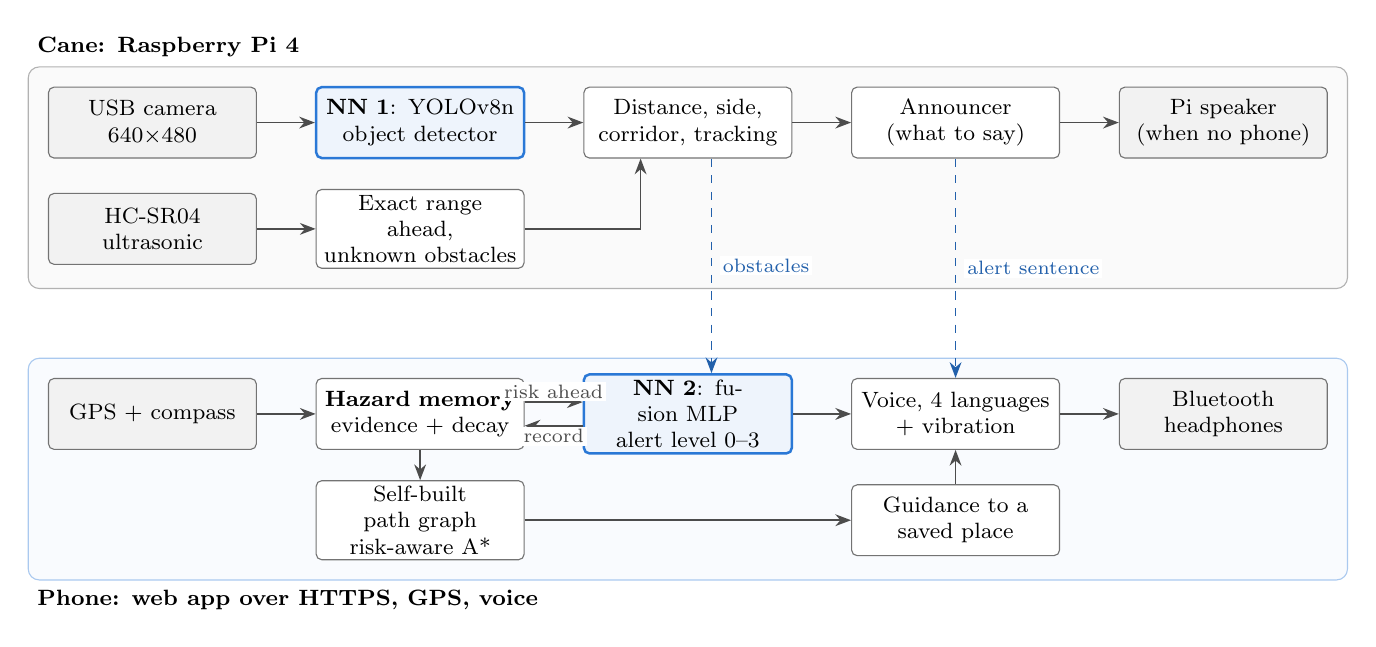
\begin{tikzpicture}[
  font=\footnotesize,
  box/.style={draw=black!55, rounded corners=2pt, fill=white, align=center, minimum height=9mm, inner sep=2pt, text width=25mm},
  nn/.style={box, draw=cblue, line width=0.9pt, fill=cblue!8},
  io/.style={box, fill=black!5},
  arr/.style={-{Stealth[length=2mm]}, black!70, line width=0.6pt},
  link/.style={arr, dashed, cblue!80!black},
  lab/.style={font=\scriptsize, fill=white, inner sep=1pt}]
  % columns 3.4 cm apart; cane rows on top, phone rows below
  \node[io]  (cam)   at (0,0)      {USB camera\\640$\times$480};
  \node[nn]  (yolo)  at (3.4,0)    {\textbf{NN 1}: YOLOv8n\\object detector};
  \node[box] (dist)  at (6.8,0)    {Distance, side,\\corridor, tracking};
  \node[box] (ann)   at (10.2,0)   {Announcer\\(what to say)};
  \node[io]  (spk)   at (13.6,0)   {Pi speaker\\(when no phone)};
  \node[io]  (us)    at (0,-1.35)  {HC-SR04\\ultrasonic};
  \node[box] (usp)   at (3.4,-1.35){Exact range ahead,\\unknown obstacles};
  \node[io]  (gps)   at (0,-3.7)   {GPS + compass};
  \node[box] (memo)  at (3.4,-3.7) {\textbf{Hazard memory}\\evidence + decay};
  \node[nn]  (fuse)  at (6.8,-3.7) {\textbf{NN 2}: fusion MLP\\alert level 0--3};
  \node[box] (voice) at (10.2,-3.7){Voice, 4 languages\\+ vibration};
  \node[io]  (hp)    at (13.6,-3.7){Bluetooth\\headphones};
  \node[box] (graph) at (3.4,-5.05){Self-built path graph\\risk-aware A*};
  \node[box] (guide) at (10.2,-5.05){Guidance to a\\saved place};
  % cane
  \draw[arr] (cam) -- (yolo); \draw[arr] (yolo) -- (dist); \draw[arr] (dist) -- (ann); \draw[arr] (ann) -- (spk);
  \draw[arr] (us) -- (usp); \draw[arr] (usp.east) -| ([xshift=-6mm]dist.south);
  % cane -> phone (secure WebSocket)
  \draw[link] ([xshift=3mm]dist.south) -- node[lab, right, xshift=1mm]{obstacles} ([xshift=3mm]fuse.north);
  \draw[link] (ann.south) -- node[lab, right, xshift=1mm]{alert sentence} (voice.north);
  % phone
  \draw[arr] (gps) -- (memo);
  \draw[arr] ([yshift=1.5mm]memo.east) -- node[lab, above]{risk ahead} ([yshift=1.5mm]fuse.west);
  \draw[arr] ([yshift=-1.5mm]fuse.west) -- node[lab, below]{record} ([yshift=-1.5mm]memo.east);
  \draw[arr] (fuse) -- (voice); \draw[arr] (voice) -- (hp);
  \draw[arr] (memo) -- (graph); \draw[arr] (graph) -- (guide); \draw[arr] (guide) -- (voice);
  \begin{scope}[on background layer]
    \node[draw=black!30, fill=black!2, rounded corners, inner sep=2.5mm, fit=(cam)(spk)(us)(usp), label={[font=\footnotesize\bfseries, anchor=south west]north west:Cane: Raspberry Pi 4}] {};
    \node[draw=cblue!40, fill=cblue!3, rounded corners, inner sep=2.5mm, fit=(gps)(hp)(graph)(guide), label={[font=\footnotesize\bfseries, anchor=north west]south west:Phone: web app over HTTPS, GPS, voice}] {};
  \end{scope}
\end{tikzpicture}
\caption{AURALIS architecture. The cane decides \emph{what} is ahead and what to say; the phone adds location, memory, routing and the user-facing voice. Dashed arrows travel over a secure WebSocket on the phone's Wi-Fi hotspot; the phone also sends its GPS position back to the cane. Neural components are outlined in blue.}
\label{fig:arch}
\end{figure*}

\subsection{Obstacle taxonomy and walking corridor}
Detections are mapped to six categories (Table~\ref{tab:taxonomy}) that decide severity, the wording of the alert, and whether the object is remembered. Moving objects are announced but never stored. A vehicle whose estimated distance stays constant for 3\,s is re-classified as a parked, static obstacle. The image is split into left, ahead and right thirds; an object is \emph{in the walking corridor} when its box overlaps the middle third and it is within 4\,m.

\begin{table}[t]
\caption{Obstacle taxonomy (from \texttt{pi/config.py})}
\label{tab:taxonomy}
\centering\footnotesize
\begin{tabular}{@{}lp{36mm}p{19mm}@{}}
\toprule
Category & Example classes & Remembered \\
\midrule
Drop & pothole, open drain, stairs down, curb & yes; STOP $<$1.5\,m \\
Raised & stairs up, speed breaker & yes \\
Static & pole, tree, wall, bench, chair, parked vehicle & yes \\
Head height & branch, signboard, high and close objects & yes \\
Moving & person, bicycle, car, auto-rickshaw, dog, cow & no \\
Zone & construction & yes \\
\bottomrule
\end{tabular}
\end{table}

\subsection{Detection (NN 1)}
The detector is YOLOv8n~\cite{yolov8} exported to ONNX and executed with ONNX Runtime~\cite{onnxruntime} on the Pi's four CPU cores, at 480\,px (or 320\,px in a fast mode). The stock COCO model~\cite{lin2014} already covers people, vehicles, animals and street furniture. Classes specific to Indian streets (pothole, open drain, stairs, curb, speed breaker) are trained with a Colab pipeline that merges public datasets with photos collected from the cane; the cane loads the custom model automatically when present. \tbd{Report the custom model: dataset size per class, mAP@0.5, precision, recall.}

An object is announced only when it is stable in at least two of the last three frames; it is repeated after 5\,s or when it comes more than 1\,m closer, and an object closer than 0.8\,m, or any drop, interrupts current speech.

\subsection{Distance from one camera}
Two geometric estimates are available. \emph{Ground-plane geometry} uses the image row $y_b$ of the box's bottom edge: with camera height $h$, downward tilt $\theta$ and focal length $f$ (in pixels),
\begin{equation}
d = \frac{h}{\tan\!\big(\theta + \arctan\frac{y_b - H/2}{f}\big)}.
\end{equation}
\emph{Known size} uses a typical real height $H_c$ per class: $d = H_c f / h_{\text{box}}$. A monocular depth network~\cite{ranftl2022} can fill in objects neither method handles, its relative depth being re-scaled to metres every frame by fitting it to the geometric estimates.

Fig.~\ref{fig:dist} shows why we default to the size estimate: with our mounting ($h=0.9$\,m, $\theta=20^\circ$, $f=554$\,px) a tilt error of only $\pm2^\circ$---easily caused by holding the cane differently---moves the ground-plane estimate by $-6.8/+7.3\%$ at 1\,m and $-11.4/+14.4\%$ at 3\,m, and the ground is not visible closer than 0.95\,m. The size estimate is independent of how the cane is held. Its error equals the error in box height plus the spread of real object heights, which we will measure (E1). For whatever is straight ahead, the forward ultrasonic ranger replaces the camera's estimate when they agree within 1\,m, and on its own announces any unrecognised obstacle within 1\,m.

\begin{figure}[t]
\centering
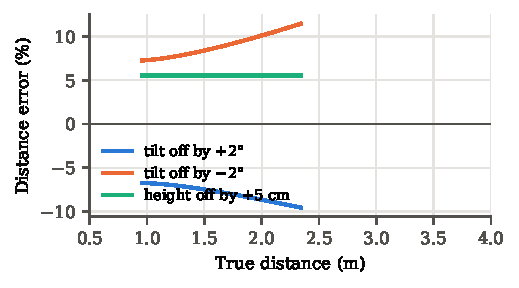
\includegraphics[width=\columnwidth]{figures/distance_sensitivity.pdf}
\caption{Error of the ground-plane distance estimate for small mounting errors (analytic, from the deployed camera parameters). The size-based estimate and the ultrasonic range do not depend on tilt.}
\label{fig:dist}
\end{figure}

% ---------------------------------------------------------------------------
\section{Spatio-Temporal Hazard Memory}\label{sec:memory}
When an alert of level \emph{warning} or higher concerns a rememberable object and the GPS fix is better than 30\,m, the hazard is stored at the user's position projected $d$ metres along the compass heading. Sightings of the same class within 8\,m are merged (position averaged with weight 3:1, at most one new sighting per minute so that standing still does not inflate the count). The risk of hazard $i$ is
\begin{equation}
r_i(t) = s_i \cdot \big(1 - e^{-n_i/2}\big) \cdot 0.5^{\,\Delta t_i / T} \cdot c_i ,
\end{equation}
where $s_i$ is the category severity, $n_i$ the number of sightings, $\Delta t_i$ the time since the last sighting, $T = 7$\,days the half-life and $c_i$ the detection confidence. One sighting gives at most 39\% of full risk, three give 78\%, five 92\%. A hazard that is no longer seen fades below the warning threshold of 0.15 after 9.7, 16.6 and 18.3 days for 1, 3 and 5 sightings (Fig.~\ref{fig:decay}). The user can also say a hazard is gone, which deletes all hazards within 10\,m.

\textbf{Early warning.} While walking, the phone looks 25\,m ahead within $\pm45^\circ$ of the heading and announces a remembered hazard once per two minutes, e.g.\ \emph{``Careful. Remembered pothole, 20 metres ahead''}. At a walking speed of 1.2\,m/s this gives about 20\,s of warning, compared with about 2.5\,s from the camera, which announces corridor obstacles within 3\,m (Table~\ref{tab:lead}).

\begin{figure}[t]
\centering
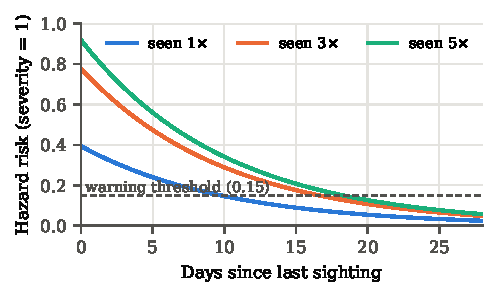
\includegraphics[width=\columnwidth]{figures/risk_decay.pdf}
\caption{Hazard risk over time without new sightings, for a hazard seen 1, 3 or 5 times (Eq.~2, severity and confidence 1). Repeated evidence keeps a hazard active for longer.}
\label{fig:decay}
\end{figure}

\begin{table}[t]
\caption{Warning distance and lead time (by design, 1.2\,m/s)}
\label{tab:lead}
\centering\footnotesize
\begin{tabular}{@{}lcc@{}}
\toprule
Source of the warning & Distance & Lead time \\
\midrule
Camera alone (announce range) & $\le 3$\,m & $\approx 2.5$\,s \\
Hazard memory (look-ahead) & $\le 25$\,m & $\approx 20.8$\,s \\
Measured in the field (E4) & \tbd{m} & \tbd{s} \\
\bottomrule
\end{tabular}
\end{table}

% ---------------------------------------------------------------------------
\section{Self-Built Map and Risk-Aware Routing}\label{sec:routing}
The phone records a breadcrumb every 5\,m walked, ignoring fixes worse than 25\,m. Breadcrumbs within 6\,m become one graph node, and consecutive nodes are joined by an edge unless they are more than 30\,m apart (a GPS jump). The result is a graph of paths the user has actually walked, with no external map. The user can name places (``Library'', ``Canteen'') by voice and ask to be guided there. Each edge $e$ of length $\ell_e$ gets the risk $\rho_e$ of the remembered hazards within 10\,m of it, and A*~\cite{hart1968} minimises
\begin{equation}
\text{cost}(e) = \ell_e \,(1 + \lambda \rho_e).
\end{equation}

On an example campus block with five remembered hazards (Fig.~\ref{fig:routing}), the shortest route ($\lambda \le 2$) is 90.8\,m long and crosses an open drain and a pothole (length-weighted risk 0.458). From $\lambda = 4$ the planner switches to a 202.7\,m detour with risk 0.051: \textbf{89\% less risk for 2.2$\times$ the distance}. The app shows both routes so the user can choose; $\lambda = 4$ is the default.

\begin{figure*}[t]
\centering
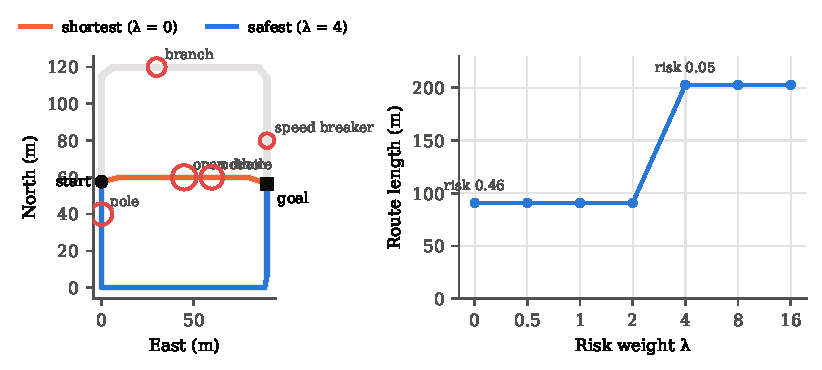
\includegraphics[width=0.78\textwidth]{figures/routing.pdf}
\caption{Risk-aware routing with the app's own code on the example campus graph. Left: shortest and safest route; circle size is hazard risk. Right: route length versus the risk weight $\lambda$, annotated with the route's length-weighted risk.}
\label{fig:routing}
\end{figure*}

% ---------------------------------------------------------------------------
\section{Neural Sensor Fusion}\label{sec:fusion}
The alert level (safe, caution, warning, urgent) is decided by a multilayer perceptron with layers $8 \to 16 \to 16 \to 4$ (ReLU, softmax; 484 parameters) that runs in the phone's browser in about 0.5\,$\mu$s per frame. Its eight inputs are: the nearest corridor obstacle's distance, the ultrasonic drop signal, the object's severity, detection confidence, box area and lateral offset, the summed risk of remembered hazards within 15\,m ahead, and the approach speed from tracking. Two safety rules sit outside the network: a drop closer than 1.5\,m is always \emph{urgent} (the network can raise but never lower this), and if the cane's data stops for more than 3\,s the phone says so and vibrates.

\textbf{Training.} Labelled field data is expensive, so the network is first trained on 20{,}000 synthetic situations labelled by an expert rule set that combines distance, threat (severity $\times$ confidence, reduced off-path), apparent size, approach speed and memory risk, with 3\% label noise; Adam~\cite{kingma2015}, 60 epochs. A \emph{research mode} in the app lets a sighted helper label real situations while walking; these rows are weighted 5$\times$ when re-training.

\textbf{Preliminary result.} On 10{,}000 fresh synthetic situations (Table~\ref{tab:fusion}, Fig.~\ref{fig:cm}) the network reaches 0.890 accuracy and 0.933 urgent recall. A distance-only rule baseline---the app's fallback when no network is loaded---reaches 0.768 and 0.865, and misses most \emph{warning} situations (recall 0.365 vs.\ 0.824), because they depend on what the object is and how it moves, not only on how far it is. We stress that these labels come from the rule teacher, so this measures how well the compact network captures a richer decision rule; field accuracy is experiment E2.

\begin{table}[t]
\caption{Fusion network vs.\ rule baseline (held-out synthetic set, $n = 10{,}000$)}
\label{tab:fusion}
\centering\footnotesize
\setlength{\tabcolsep}{4pt}
\begin{tabular}{@{}lcccc@{}}
\toprule
Model & Acc. & Macro F1 & Urgent rec. & Urgent prec. \\
\midrule
Distance rules & 0.768 & 0.754 & 0.865 & 0.988 \\
Fusion MLP & \textbf{0.890} & \textbf{0.890} & \textbf{0.933} & 0.917 \\
Field data (E2) & \tbd{} & \tbd{} & \tbd{} & \tbd{} \\
\bottomrule
\end{tabular}
\end{table}

\begin{figure}[t]
\centering
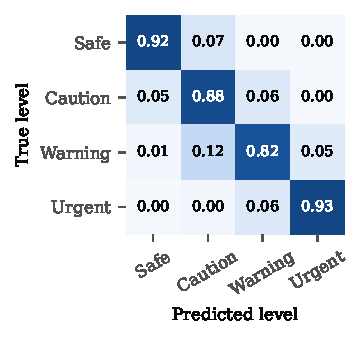
\includegraphics[width=0.66\columnwidth]{figures/fusion_confusion.pdf}
\caption{Row-normalised confusion matrix of the fusion network on the held-out synthetic set. Only 7 of 1{,}194 urgent situations (0.6\%) are predicted as safe or caution; most errors are between neighbouring levels.}
\label{fig:cm}
\end{figure}

% ---------------------------------------------------------------------------
\section{Implementation}
The cane software is Python (OpenCV, ONNX Runtime, aiohttp) and starts with one command; it serves the phone application, the annotated camera stream for a helper and the memory store. The phone application is a responsive web app (Fig.~\ref{fig:app}) with four screens---Walk, Places, Memory, Settings---fully translated into English, Hindi, Telugu and Tamil. Speech uses neural text-to-speech voices on the Pi, cached for offline use, or the phone's own voices; when a phone is connected the alerts are spoken on the phone, so that they reach the user's Bluetooth headphones, and the Pi speaker falls silent. Holding a hand in front of the ultrasonic sensor for 2\,s pauses or resumes the cane without touching the phone. The map uses Leaflet with OpenStreetMap tiles~\cite{haklay2008}; paths, hazards and places are still drawn when offline.

On a development laptop CPU the detector takes 10.5\,ms (320\,px) and 22.4\,ms (480\,px) per frame. \tbd{Measure on the Pi 4: detector latency, end-to-end frames per second, and alert latency (E3).}

\begin{figure*}[t]
\centering
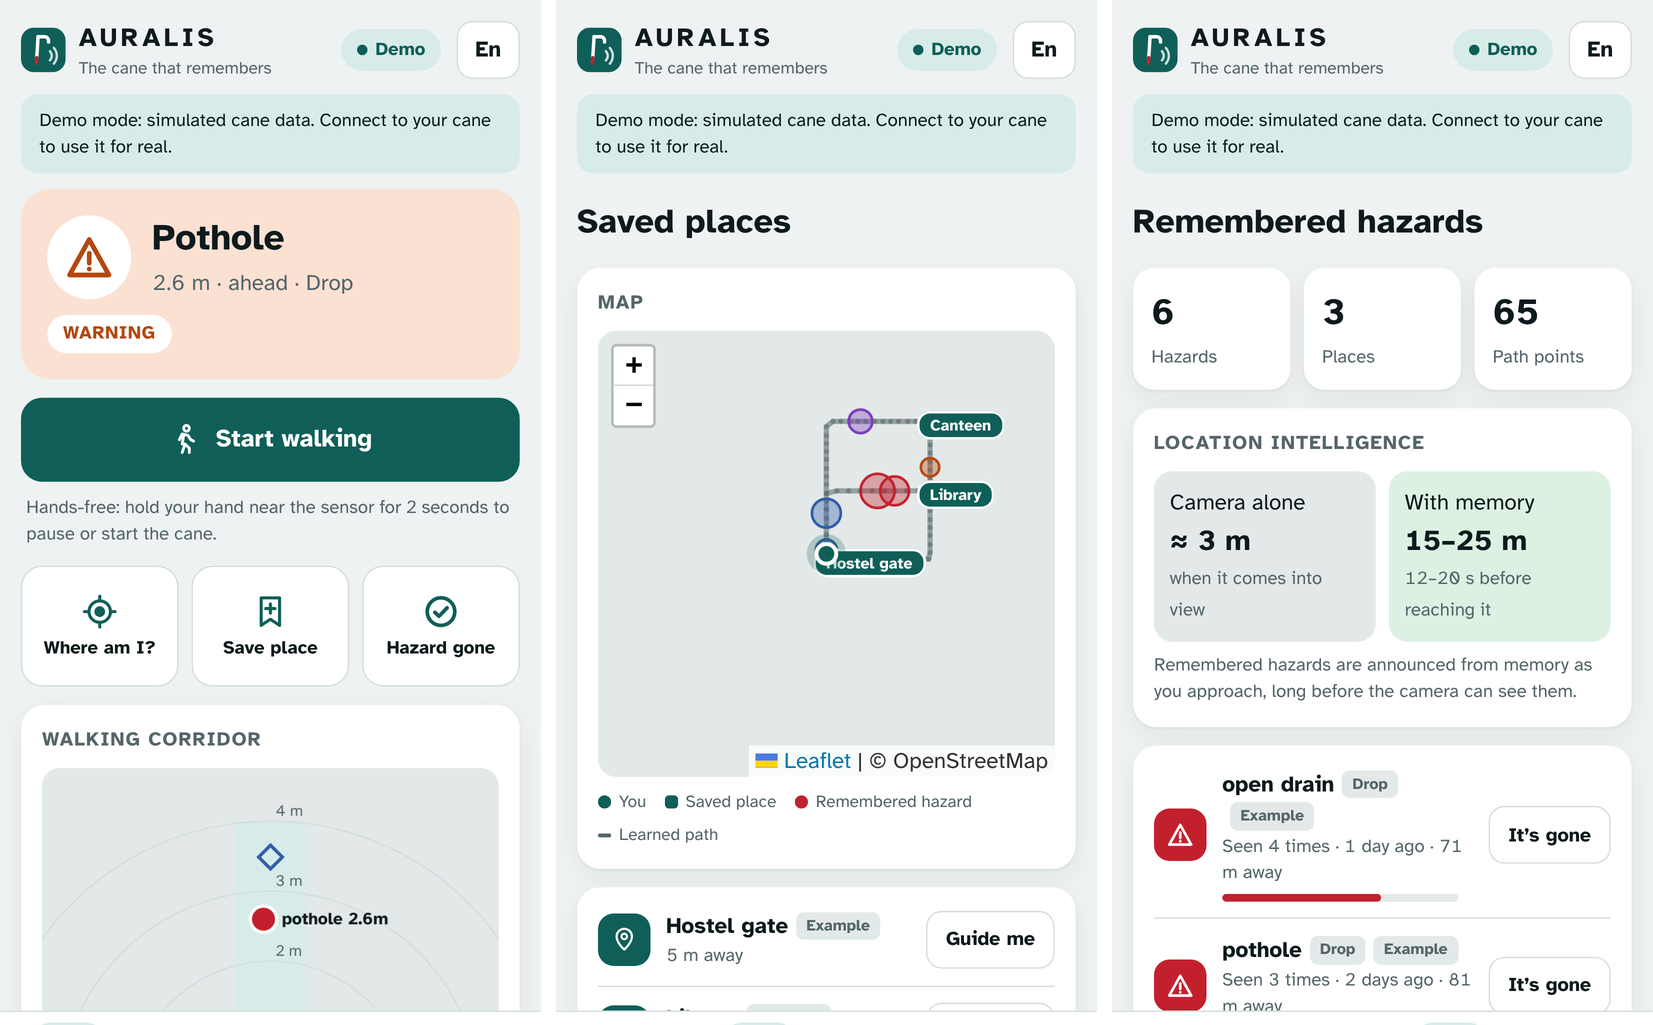
\includegraphics[width=0.82\textwidth]{figures/app_screens.png}
\caption{Phone application (demo mode with simulated sensor data, map background not loaded). Left: Walk screen with the current alert and the top-down walking corridor; the hollow diamond is a remembered hazard ahead. Middle: self-built path graph with remembered hazards and saved places. Right: hazard memory with evidence counts, age and risk.}
\label{fig:app}
\end{figure*}

% ---------------------------------------------------------------------------
\section{Planned Evaluation}
Table~\ref{tab:plan} lists the field experiments that complete this study. All of them can be run on campus with the existing hardware and the app's research mode and log export.

\begin{table}[t]
\caption{Field experiments (to be completed)}
\label{tab:plan}
\centering\footnotesize
\begin{tabular}{@{}lp{38mm}l@{}}
\toprule
\# & Experiment & Metric \\
\midrule
E1 & Distance vs.\ tape measure at 0.5/1/2/3\,m, 10 readings each, size vs.\ ground vs.\ ultrasonic & MAE, std \\
E1c & Custom detector on held-out campus photos & P, R, mAP@0.5 \\
E2 & Fusion network vs.\ rules on labelled walks (80/20) & accuracy, urgent recall \\
E3 & Obstacle appears $\to$ voice starts (video) & latency (ms) \\
E4 & Walk one route 5$\times$ past a fixed hazard & warning distance, lead time \\
E5 & Shortest vs.\ safest on two real campus routes & length, risk \\
E7 & 5 listeners rate each language & intelligibility (1--5) \\
\bottomrule
\end{tabular}
\end{table}

% ---------------------------------------------------------------------------
\section{Limitations and Future Work}
GPS accuracy (typically 5--10\,m outdoors, worse near buildings) limits where a remembered hazard can be placed; merging repeated sightings and the 8\,m merge radius partly compensate. Indoors there is no GPS, and memory only works outdoors. The fusion network is so far trained on synthetic data, and the stock detector does not yet know potholes, drains and stairs; both are addressed by the planned field data. Memory is per user; sharing anonymised hazards between users of the same campus would let one user's sighting protect others, and is our main next step, together with a native app that keeps working with the screen off.

\section{Conclusion}
AURALIS shows that a commodity smart cane can do more than react: by remembering where hazards are, learning the user's own paths and fusing what it sees with what it remembers, it can warn several times earlier and route around known dangers, while keeping the hardware to one board, one camera and one ultrasonic sensor, and the user's own phone and headphones.

\section*{Acknowledgment}
\tbd{Guide, department and lab.}

% Verify every entry against the original before submission.
\begin{thebibliography}{99}\footnotesize
\bibitem{who2019} World Health Organization, \emph{World Report on Vision}. Geneva, Switzerland: WHO, 2019.
\bibitem{bourne2017} R. R. A. Bourne \emph{et al.}, ``Magnitude, temporal trends, and projections of the global prevalence of blindness and distance and near vision impairment: a systematic review and meta-analysis,'' \emph{Lancet Global Health}, vol.~5, no.~9, pp.~e888--e897, 2017.
\bibitem{dakopoulos2010} D. Dakopoulos and N. G. Bourbakis, ``Wearable obstacle avoidance electronic travel aids for blind: a survey,'' \emph{IEEE Trans. Syst., Man, Cybern. C}, vol.~40, no.~1, pp.~25--35, 2010.
\bibitem{elmannai2017} W. Elmannai and K. Elleithy, ``Sensor-based assistive devices for visually-impaired people: current status, challenges, and future directions,'' \emph{Sensors}, vol.~17, no.~3, p.~565, 2017.
\bibitem{real2019} S. Real and A. Araujo, ``Navigation systems for the blind and visually impaired: past work, challenges, and open problems,'' \emph{Sensors}, vol.~19, no.~15, p.~3404, 2019.
\bibitem{kuriakose2022} B. Kuriakose, R. Shrestha, and F. E. Sandnes, ``Tools and technologies for blind and visually impaired navigation support: a review,'' \emph{IETE Tech. Rev.}, vol.~39, no.~1, pp.~3--18, 2022.
\bibitem{redmon2016} J. Redmon, S. Divvala, R. Girshick, and A. Farhadi, ``You only look once: unified, real-time object detection,'' in \emph{Proc. IEEE CVPR}, 2016, pp.~779--788.
\bibitem{yolov8} G. Jocher, A. Chaurasia, and J. Qiu, ``Ultralytics YOLOv8,'' 2023. [Online]. Available: https://github.com/ultralytics/ultralytics
\bibitem{lin2014} T.-Y. Lin \emph{et al.}, ``Microsoft COCO: common objects in context,'' in \emph{Proc. ECCV}, 2014, pp.~740--755.
\bibitem{ranftl2022} R. Ranftl, K. Lasinger, D. Hafner, K. Schindler, and V. Koltun, ``Towards robust monocular depth estimation: mixing datasets for zero-shot cross-dataset transfer,'' \emph{IEEE Trans. Pattern Anal. Mach. Intell.}, vol.~44, no.~3, pp.~1623--1637, 2022.
\bibitem{saha2019} M. Saha \emph{et al.}, ``Project Sidewalk: a web-based crowdsourcing tool for collecting sidewalk accessibility data at scale,'' in \emph{Proc. ACM CHI}, 2019.
\bibitem{haklay2008} M. Haklay and P. Weber, ``OpenStreetMap: user-generated street maps,'' \emph{IEEE Pervasive Comput.}, vol.~7, no.~4, pp.~12--18, 2008.
\bibitem{hart1968} P. E. Hart, N. J. Nilsson, and B. Raphael, ``A formal basis for the heuristic determination of minimum cost paths,'' \emph{IEEE Trans. Syst. Sci. Cybern.}, vol.~4, no.~2, pp.~100--107, 1968.
\bibitem{kingma2015} D. P. Kingma and J. Ba, ``Adam: a method for stochastic optimization,'' in \emph{Proc. ICLR}, 2015.
\bibitem{onnxruntime} ONNX Runtime developers, ``ONNX Runtime,'' 2021. [Online]. Available: https://onnxruntime.ai
\end{thebibliography}

\end{document}
